\chapter{Background}
\label{sec:background}
  In this section, the theoretical background of the project and used technologies are described. First the Eclipse Foundation is introduced, as many used frameworks are developed under the Eclipse Foundation. Then, the Eclipse Modeling Framework is described, as it is the core of the used frameworks. After that, the model transformation language Henshin is introduced. Finally, the framework \ac{glsp} is described, that is used to create web-based diagram editors.

  \section{Eclipse Foundation}
  \label{subsec:eclipse-foundation}
  The Eclipse Foundation is a not-for-profit, member-supported corporation that provides an environment for individuals and organizations for collaborative and innovative software development. \cite{eclipse-review} The Eclipse Foundation grew out of the publication of the Eclipse \ac{ide} code from IBM in 2001. The Eclipse Foundation itself was founded in 2004. The new organization was founded to continue the development of Eclipse IDE as an open source platform. Over time, the organization initiated numerous projects in the Eclipse environment, all operating under the Eclipse Public License. \cite{heise-eclipse-foundation,eclipse-review} In the recent years, the key initiatives of the Eclipse Foundation are contributing to european digital sovereignty, enhancing security measures, innovating \ac{sdv}, organizing community events, and improving their most popular projects. Popular projects are for example the Jakarta EE, an ecosystem for cloud-native applications with java, Eclipse Temurin, providing open source Java Development Kits and the Eclipse IDE. \cite{eclipse-report} In total, the Eclipse Foundation hosts more than 400 open source projects, supported 14 european research projects in 2024, and has 117 organizations participating in commits. \cite{eclipse-report}

  The scope of this work remains within the Eclipse Foundation ecosystem. All frameworks used are projects from the Eclipse Foundation. The used frameworks are described in the sections \ref{subsec:emf}, \ref{subsec:henshin} and \ref{subsec:glsp}.

  The Eclipse \ac{ide} is not the main project, but it is still an important part of the Eclipse infrastructure. It is divided into four main components: Equinox, the Platform, the \ac{jdt} and the \ac{pde}. Together they provide everything to develop and extend Eclipse-based tools. Equinox and the Platform are the core of the Eclipse \ac{ide}. With expanding the core with the \ac{jdt} or other plugins, the \ac{ide} can be used to develop different programming languages, like Java, C/C++, or PHP. \cite{emf} Eclipse provides different packages to download, depending on the use case. One package is the Eclipse Modeling Tools package by the Eclipse Modeling Project. It provides tools and runtimes to build model-based applications. It can be used to graphically design domain models and test those models by creating and editing dynamic instances. Also, Java code can be generated from the models to get a scaffold that can be used to create applications on top. \cite{eclipse_modeling} The base of the Eclipse Modeling Tool is \ac{emf} (section \ref{subsec:emf}). Other modeling tools and projects that are built on top of the \ac{emf} core functionality provide capabilities for model transformation, database integration, or graphical editor generation. \cite{emf}

  \section{\acf{emf}}
    \label{subsec:emf}

    \begin{quote}
      \glqq\acf{emf} is a modeling framework and code generation facility for building tools and other applications based on a structured data model.\grqq{} \autocite{emf-repo}
    \end{quote}

    \acf{emf} is the core part of the Eclipse Modeling Project and unifies the representation of models in \acs{uml}, \acs{xml} and Java. You can define your model in one of these formats and use \ac{emf} to generate the other formats.
    
    \ac{emf} consists of three components. The \ac{emf} core part provides Ecore metamodels, runtime support for the models, and a basic \acs{api} for manipulating \ac{emf} objects generically. Ecore metamodels are used to describe the structure of a model. \cite{eclipse_emf} They can be serialized in \ac{xmi} 2.0, as Ecore \ac{xmi}, and have the file extension \textit{.ecore}. There are several Ecore classes to represent a model, here are the most important ones:

    \begin{itemize}
      \item \textbf{EClass}: A class in the model that is identified by a name, containing attributes and references to other classes. It can also refer to a number of other classes as its supertypes to support inheritance. \cite{emf}
      \item \textbf{EAttribute}: An attribute of a class, that are identified by a name and have a type. \cite{emf}
      \item \textbf{EDataType}: A simple data type like \code{EString}, \code{EBoolean} or \code{EJavaClass}. \cite{emf}
      \item \textbf{EReference}: A reference to another class, containing a link to an instance of that class. \cite{emf}
    \end{itemize}


    Together, \citeauthor{emf} called these classes the Ecore kernel. In Figure \ref{fig:emf-kernel} you can see the kernel classes and their relations. These classes are enough to define simple models. \textbf{EAttribute} and \textbf{EReference} have a lot of similarities. They both define the state of an instance of an \textbf{EClass} and have a name and a type. For that, Ecore provides a common interface for both, called \textbf{EStructuralFeature}. Ecore can also model behavioral features of classes as \textbf{EOperation} using \textbf{EParameter}. All classes have the common interface \textbf{EObject}, being the root of all modeled objects. Related classes are grouped into packages called \textbf{EPackage}. It is represented by the root element when the model is serialized. \cite{emf}

    \begin{figure}[h]
      \centering
      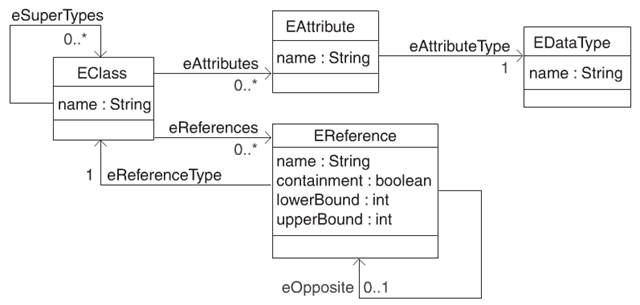
\includegraphics[width=0.7\textwidth]{emf-kernel}
      \caption{The Ecore kernel. Image obtained from \cite{emf}}
      \label{fig:emf-kernel}
    \end{figure}

    The second component of \ac{emf} is \ac{emf}.Edit. It provides generic reusable classes to build viewers and editors for \ac{emf} models. With these classes, \ac{emf} metamodels can be displayed in JFace viewers, that are part of the Eclipse \acs{ui}. \cite{eclipse_emf} The Eclipse \ac{ide} can display an Ecore model in a tree viewer. Eclipse accesses the data over the \code{ITreeContentProvider} interface to navigate the content and the \code{ILabelProvider} interface to provide the label text and icons for the displayed objects. The properties of objects are displayed in a Property Sheet over the \code{IPropertySourceProvider}, where the user can edit the model. \ac{emf}.Edit also provides undo and redo operations when creating or editing an instance model. For that, it uses a command framework with commands like an \code{AddCommand}, \code{SetCommand} or \code{CopyCommand}. \cite{emf}

    The third component is \ac{emf}.Codegen. It can generate Java code for a complete editor for \ac{emf} instance models of an Ecore metamodel. It provides different generation options. So, unlike \ac{emf}.Edit, that just provides generic classes for Ecore models, \ac{emf}.Codegen directly generates complete editors with a \acs{ui}. \cite{eclipse_emf} The generation can be done over a wizard in the Eclipse \ac{ide} or by using the command line interface. \cite{emf} The generation can be separated into three levels. The first level is to generate Java interfaces and implementations for the Ecore model classes and a factory- and package-implementation class. The second level generates specific \code{ItemProviders} to edit instance models based on the metamodel. The classes are structured like the \ac{emf}.Edit component for the Ecore models. The third level generates a structured editor with \acs{ui} that works like the Ecore editor in the Eclipse \ac{ide} and can be a starting point for customization. \cite{eclipse_emf} There are many frameworks that build on top of \ac{emf}, using these generation capabilities to create further modeling functionality. For model transformations the most popular frameworks that build upon \ac{emf} are Eclipse Acceleo, Eclipse VIATRA, Eclipse ATL, Eclipse QVT Operational, Eclipse QVT Declarative and Henshin \ref{subsec:henshin}.

  \section{Henshin}
  \label{subsec:henshin}

  One part of the Eclipse Modeling Project for model transformations is Henshin. It can be used as a plugin in the Eclipse \ac{ide} or as an \acs{sdk}. It provides a graphical and textual syntax to define model transformation rules and apply them to \ac{emf} XMI instance models. It can be used for endogenous transformations, where \ac{emf} model instances are directly transformed, and exogenous transformations, where new instances are generated from given instances using a trace model. It also brings efficient in-place execution of transformations using an interpreter with debugging support and a performance profiler. Henshin also provides conflict and dependency analysis, and state space analysis for verification. \cite{henshin-repo}

  Henshin builds on top of \ac{emf}. It uses an Ecore metamodel to define the structure of the transformation rules, resulting in a serialized \ac{xmi} file with the file extension \textit{.hensin}, that can therefore be edited in the Eclipse tree editor. \cite{henshin-repo} The metamodel of the transformation rules uses another Ecore metamodel that models the model structure of the domain, to type the nodes, egdes, and attributes of the rules. \cite{henshin} In Figure \ref{fig:henshin-rule-model} you can see the Henshin transformation rule metamodel. A rule consists of a \ac{rhs} graph, a \ac{lhs} graph and attribute conditions. Additionally, mappings between the \ac{lhs} and \ac{rhs} graph are defined between nodes. The mapping of the edges is done implicitly by the mapping of the source and target nodes. \cite{henshin} Henshin uses units to control the order of rule applications. With units, control structures can be defined. Also, parameters can be passed from the previous executed rule to the next one to have a controlled object flow. Henshin's tansformation language is based on algebraic graph transformations, complying with the syntactical and semantic structure of rules and transformation units. This ensures a language usable for formal verification or validation. \cite{henshin}

  In the Eclipse \ac{ide}, rules can also be edited in a graphical editor. The rules are displayed as a single graph, calculated from the \ac{lhs} and \ac{rhs} graphs. The nodes and edges are annotated with \textit{\textless{}\textless{}preserve\textgreater\textgreater}, \textit{\textless{}\textless{}create\textgreater\textgreater}, \textit{\textless{}\textless{}delete\textgreater\textgreater}, \textit{\textless{}\textless{}forbid\textgreater\textgreater} or \textit{\textless{}\textless{}require\textgreater\textgreater} to indicate what happens to the nodes and edges when applying the rule. These annotations can be directly edited in the graphical editor and the the \ac{lhs} and \ac{rhs} graphs are then adapted to the change. Also, multiple \acp{nac}, \acp{pac} and parameters can be specified directly. \cite{henshin-repo} When a set of transformation rules are specified, they can be applied to an \ac{emf} \ac{xmi} instance model, by using a wizard in the Eclipse \ac{ide}. There, the source model, the rule, and its parameters can be selected. The result of the transformation can be seen in a new \ac{xmi} instance file. \cite{henshin-repo} Next to the graphical editor, Henshin also provides a textual syntax to define transformation rules and units. In a \textit{.henshin\_rule} file with the keyword \textbf{rule} a name and parameters, a new rule can be described. If you want to define a node, you can use the keyword \textbf{node} with a action keyword like \textbf{create} or \textbf{preserve} to specify the action of the node in the transformation. 

  The Henshin \acs{sdk} consists of multiple packages oriented to the package structure of \ac{emf}. Next to a model, edit, and editor package, it provides an interpreter package, that contains a default engine to execute model transformations.

  \begin{figure}[h]
    \centering
    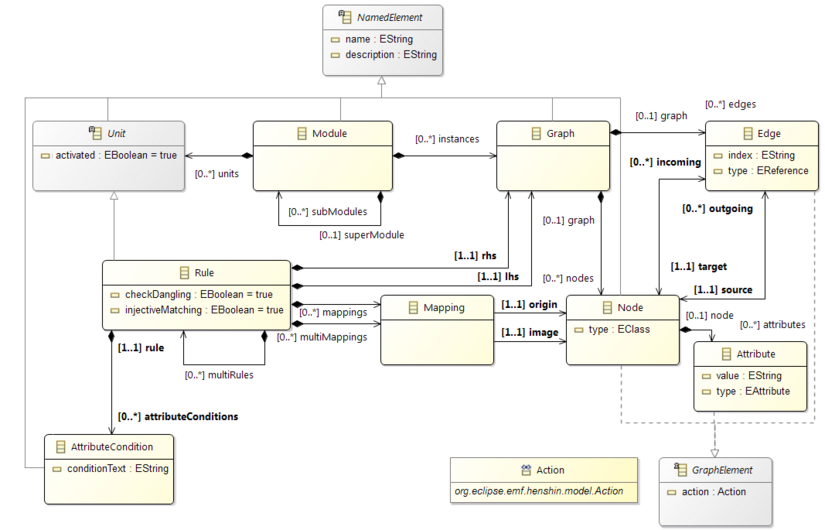
\includegraphics[width=1\textwidth]{henshin-rule-model}
    \caption{Henshin transformation rule metamodel. Image obtained from \cite{henshin-repo}}
    \label{fig:henshin-rule-model}
  \end{figure}

  \section{\acf{glsp}}
  \label{subsec:glsp}

  \ac{glsp} is a framework that provides components for the development of \acsp{gui} for web-based diagram editors.
  \cite{glsp-repo} It is organized within the Eclipse Cloud Development project. \cite{glsp-doc} With the framework, custom diagram editors for Eclipse Theia, Eclipse IDE, Visual Studio Code, or standalone web apps can be created. It uses a client-server architecture, where the client is implemented with TypeScript and for the server, GLSP provides implementations in Java and TypeScript based on nodejs, even though the server could be implemented in any programming language. As the server for this project is implemented in Java, the following discussion focuses exclusively on the Java implementation of the \ac{glsp} server. Client and server communicate over JSON-\acs{rpc} with an action protocol that is similar to the Language Server Protocol \cite{lsp-repo}. 

  The \ac{glsp} server is responsible for loading a source model and defines how to transform it into the graphical model, that should be displayed. The source model can be of any format, e.g., a database, JSON file, or an EMF model. \ac{glsp} provides dedicated modules for loading EMF models. The Java server uses Google Guice \cite{guice-repo} for \ac{di}. The \ac{glsp} server distinguishes between \ac{di} containers. There is one server \ac{di} container to configure global components that are not related to specific sessions. For every client session, there is a diagram session \ac{di} container, that holds session specific information, handlers, and states associated with a single diagram language. In Figure \ref{fig:glsp-server-di} you can see that the diagram session \ac{di} container run inside the server \ac{di} container. \ac{glsp} provides some abstract base classes that have to be implemented to create a working diagram server language, that can provide a diagram to display at the client. All concrete implementations of one diagram language have to be registered in a \code{DiagramModule}. The server can handle multiple diagram languages by providing different diagram modules. There are some classes that have to be implemented. The interface \code{SourceModelStorage} defines how to load and save the source model. There is already a default abstract implementation for \ac{emf} models, that loads the \ac{xmi} file into a \code{ResourceSet}. The interface \code{GModelFactory} is used to map the source model to the \ac{glsp} internal graphical model structure. Here also an abstract \code{EMFGModelFactory} is provided. Another important part is the \code{GModelState} interface, that defines the state of a client session and holds all information about the current state of the original source model. All services and handlers use the \code{GModelState} to obtain required information for their tasks.

   \begin{figure}[h]
    \centering
    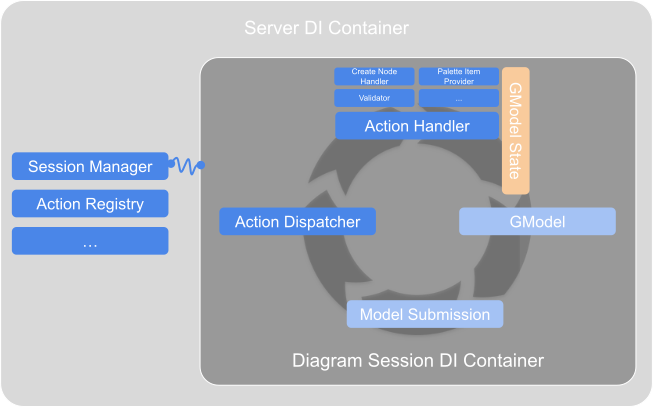
\includegraphics[width=0.7\textwidth]{glsp-server-di}
    \caption{Server DI Container vs Diagram Session DI Container. Image obtained from \cite{glsp-doc}}
    \label{fig:glsp-server-di}
  \end{figure}

  When the diagram should be displayed in the editor, the client sends a \code{RequestModelAction} with a \acs{uri} of the source model to the server. The server invokes the \code{SourceModelStorage} to load the source model and then uses the \code{GModelFactory} to translate it into the graphical model, which is then sent to the client to render it. For an edit operation, the client sends the operation request to the server, where the corresponding handler is invoked. The handler modifies the source model directly. After that, the server invokes the \code{GModelFactory} again to map the newly modified source model into a new graphical model, which is sent to the client to re-render. The two use cases share many steps. Since a new graphical model is created every time, the format of the source model is independent and can be of any format. \cite{glsp-doc}

  The \ac{glsp} client is responsible for rendering the graph and managing user interactions. The client requests all possible editing operations that can be performed on the specific model. As the client for this project is integrated into Eclipse Theia, the following discussion focuses exclusively on the Theia integration of the \ac{glsp} client. \cite{glsp-doc} \ac{glsp} provides four main \acs{ui} components to apply commands or edit the graph but also allows custom \ac{ui} extensions: 

  \begin{itemize}
    \item \textbf{ToolPalette}: The ToolPalette is an expandable \ac{ui} element located on the top left of the diagram editor. By default, it provides basic options to switch between selection, deletion, and marquee tools, validate the model, reset the viewport, and search in the listed operations below. Below it lists all nodes and edges that can be created in the diagram by default. It can be extended with custom actions by implementing and registering the \code{ToolPaletteItemProvider} interface at the server. \cite{glsp-doc,glsp-repo} 
    \item \textbf{CommandPalette}: The CommandPalette can be invoked by pressing \textit{Ctrl+Space}. It provides a search field to search for commands or actions that were registered. Commands can be registered by implementing and registering the \code{CommandPaletteActionProvider} to the server or implementing and registering the \code{CommandContribution} interface to the Theia frontend module. \cite{glsp-doc,glsp-repo} 
    \item \textbf{ContextMenu}: The ContextMenu is a popup menu that can be opened by right clicking inside the diagram editor. There, any commands or actions can be structured as needed. It can be customized by implementing and registering the \code{ContextMenuItemProvider} to the server or implementing and registering the \code{MenuContribution} interface to the Theia frontend module. \cite{glsp-doc,glsp-repo} 
    \item \textbf{EditLabelUI}: Labels of nodes and edges can be edited by double-clicking on the label. The EditLabelUI provides an input popup to edit the label text. \cite{glsp-doc,glsp-repo}
    \item \textbf{Custom \acs{ui} Components}: Custom \acs{ui} extensions have to extend \code{AbstractUIExtension} that provides a base \acs{html} element and can then be registered to the client. The base class also provides functionality to show, hide, or focus the element. These \acs{ui} extensions can also be enabled over a \code{SetUIExtensionVisibilityAction} from the server. \cite{glsp-doc,glsp-repo}
  \end{itemize}

  \ac{glsp} uses Sprotty \cite{sprotty-repo}, a web-\acs{svg}-based diagramming framework, to render the diagrams. The graphical model of \ac{glsp} called \textit{GModel} is based on the \textit{SModel} of Sprotty and works as a compatible extension. The graphical model is composed of shape elements and edges. They are organized in a tree, that starts with the \code{GModelRoot}. There are several base classes, that can be extended and also new types can be added. The \code{GEdge} represents an edge between two nodes or ports. Four classes inherit from \code{GShapeElement}, which represents an element with a certain shape, position, and size. They can also be nested inside another \code{GShapeElement}. The \code{GNode} can have \code{GLabel} or \code{GPort}, which represents a connection point for edges, as children. The \code{GCompartment} can be used as a generic container to group elements. The Java server uses \ac{emf} to handle the graphical model internally, to profit from the command-based editing capabilities of \ac{emf}. To send the graphical model to the client, it is serialized into JSON using GSON \cite{gson-repo} and then sent over JSON-\acs{rpc}. \cite{glsp-doc}

  The layout of a graph is divided into macro and micro layouting.
  The macro layouting, which arranges the nodes and edges of the model, is done by the server. The client does the micro layouting by calculating the positioning and size of elements within a container element. \cite{glsp-doc} For the macro layouting, \ac{glsp} provides a notation model, that persists the position and size of the elements in a separate notation \ac{xmi} file. The notation diagram can be added to the \code{GModelState} and then used in the \code{GModelFactory} to specify the layout. \cite{glsp-repo} \ac{glsp} also provides a \code{LayoutEngine} interface, that can be used to layout the elements of a graph that have no persisted layout yet. \cite{glsp-doc}

  \ac{glsp} also provides an interface to validate the model. With the \code{ModelValidator} interface, specific validation rules can be defined by the server. The validation returns a list of markers that can be an info, warning, or error. The markers are then displayed in the \ac{glsp} client. The markers can also be integrated into the Theia Problems View.
